\section{Soluzione}

Si è scelto di realizzare un riconoscitore della sequenza 1011001, il cui automa a stati finiti è rappresentato in \textit{Figura~\ref{fig:fsmMoore}}.

\begin{figure}[ht]
\begin{centering}
\begin{center}
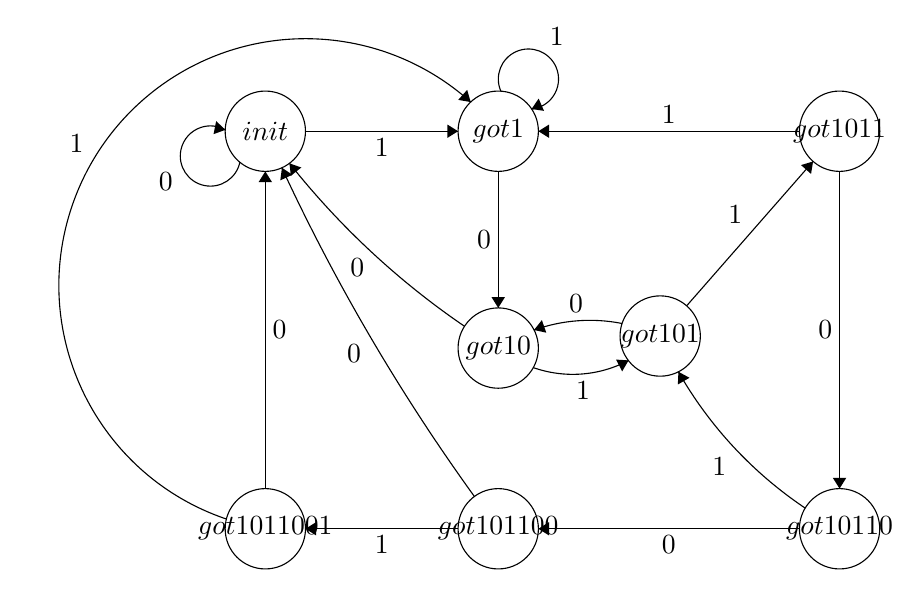
\begin{tikzpicture}[scale=0.17]
\tikzstyle{every node}+=[inner sep=0pt]
\draw [black] (16.9,-19.6) circle (3);
\draw (16.9,-19.6) node {$init$};
\draw [black] (34.3,-19.6) circle (3);
\draw (34.3,-19.6) node {$got1$};
\draw [black] (34.3,-35.8) circle (3);
\draw (34.3,-35.8) node {$got10$};
\draw [black] (46.4,-34.9) circle (3);
\draw (46.4,-34.9) node {$got101$};
\draw [black] (59.8,-19.6) circle (3);
\draw (59.8,-19.6) node {$got1011$};
\draw [black] (59.8,-49.3) circle (3);
\draw (59.8,-49.3) node {$got10110$};
\draw [black] (34.3,-49.3) circle (3);
\draw (34.3,-49.3) node {$got101100$};
\draw [black] (16.9,-49.3) circle (3);
\draw (16.9,-49.3) node {$got1011001$};
\draw [black] (19.9,-19.6) -- (31.3,-19.6);
\fill [black] (31.3,-19.6) -- (30.5,-19.1) -- (30.5,-20.1);
\draw (25.6,-20.1) node [below] {$1$};
\draw [black] (15.001,-21.908) arc (-11.7124:-299.7124:2.25);
\draw (10.02,-23.38) node [left] {$0$};
\fill [black] (13.91,-19.5) -- (13.23,-18.84) -- (13.03,-19.82);
\draw [black] (34.3,-22.6) -- (34.3,-32.8);
\fill [black] (34.3,-32.8) -- (34.8,-32) -- (33.8,-32);
\draw (33.8,-27.7) node [left] {$0$};
\draw [black] (34.5,-16.618) arc (203.9028:-84.0972:2.25);
\draw (38.68,-13.26) node [above] {$1$};
\fill [black] (36.79,-17.94) -- (37.72,-18.08) -- (37.32,-17.16);
\draw [black] (31.78,-34.172) arc (-124.30564:-141.60355:59.408);
\fill [black] (18.7,-22) -- (18.81,-22.93) -- (19.59,-22.31);
\draw (23.77,-29.06) node [below] {$0$};
\draw [black] (44.037,-36.725) arc (-62.01055:-109.48177:8.88);
\fill [black] (44.04,-36.72) -- (43.1,-36.66) -- (43.56,-37.54);
\draw (40.64,-38.3) node [below] {$1$};
\draw [black] (36.973,-34.454) arc (109.77074:78.73693:12.341);
\fill [black] (36.97,-34.45) -- (37.89,-34.65) -- (37.56,-33.71);
\draw (40.12,-33.19) node [above] {$0$};
\draw [black] (48.38,-32.64) -- (57.82,-21.86);
\fill [black] (57.82,-21.86) -- (56.92,-22.13) -- (57.67,-22.79);
\draw (52.56,-25.8) node [left] {$1$};
\draw [black] (56.8,-19.6) -- (37.3,-19.6);
\fill [black] (37.3,-19.6) -- (38.1,-20.1) -- (38.1,-19.1);
\draw (47.05,-19.1) node [above] {$1$};
\draw [black] (59.8,-22.6) -- (59.8,-46.3);
\fill [black] (59.8,-46.3) -- (60.3,-45.5) -- (59.3,-45.5);
\draw (59.3,-34.45) node [left] {$0$};
\draw [black] (56.8,-49.3) -- (37.3,-49.3);
\fill [black] (37.3,-49.3) -- (38.1,-49.8) -- (38.1,-48.8);
\draw (47.05,-49.8) node [below] {$0$};
\draw [black] (57.23,-47.754) arc (-123.85357:-150.26665:30.434);
\fill [black] (47.76,-37.57) -- (47.72,-38.52) -- (48.59,-38.02);
\draw (51.37,-44.68) node [left] {$1$};
\draw [black] (31.3,-49.3) -- (19.9,-49.3);
\fill [black] (19.9,-49.3) -- (20.7,-49.8) -- (20.7,-48.8);
\draw (25.6,-49.8) node [below] {$1$};
\draw [black] (32.519,-46.886) arc (-144.15959:-155.11187:149.088);
\fill [black] (18.14,-22.33) -- (18.02,-23.27) -- (18.93,-22.85);
\draw (24.09,-36.2) node [left] {$0$};
\draw [black] (16.9,-46.3) -- (16.9,-22.6);
\fill [black] (16.9,-22.6) -- (16.4,-23.4) -- (17.4,-23.4);
\draw (17.4,-34.45) node [right] {$0$};
\draw [black] (13.993,-48.572) arc (-108.72779:-312.00075:18.431);
\fill [black] (32.24,-17.42) -- (31.98,-16.51) -- (31.31,-17.26);
\draw (3.36,-20.56) node [left] {$1$};
\end{tikzpicture}
\end{center}
\par\end{centering}
\caption{\label{fig:fsmMoore}Macchina di Moore}
\end{figure}



Inizialmente, si è utilizzato un automa di Moore ed è stata effettuata la sua descrizione behavioral a doppio processo. Sebbene la soluzione a singolo processo sia più compatta, si è preferita la realizzazione a doppio processo perché aderisce perfettamente alla struttura di una macchina a stati finiti. In ogni caso, è opportuno osservare che la soluzione a singolo processo viene generalmente preferita perché in FSM complesse, se realizzate a doppio processo, la sensitivity list del processo che descrive la parte combinatoria è molto grande e aumenta la probabilità di errore nello scrivere il codice, ed inoltre si può facilmente incorrere in problemi dovuti all'effetto memoria di assegnazioni incomplete di variabili, segnalati da ISE tramite warning di questo tipo:

\begin{framed} 
\textit{WARNING:Xst:737 - Found 1-bit latch for signal <Q\_0>. Latches may be generated from incomplete case or if statements. We do not recommend the use of latches in FPGA/CPLD designs, as they may lead to timing problems.}
\end{framed}


L'interfaccia del riconoscitore di sequenza, il cui codice è nella cartella \lstinline{Esercizio_07/sequence_recognizer/}, è la seguente:

\begin{lstlisting}[language=VHDL,caption={Interfaccia del riconoscitore di sequenza}] 
entity sequence_recognizer is
    Port ( clk : in  STD_LOGIC;
           value_in : in  STD_LOGIC;
           value_out : out  STD_LOGIC);
end sequence_recognizer;
\end{lstlisting}\selectlanguage{italian}%

Il componente realizzato analizza, su ogni fronte di salita del clock, il valore di \lstinline{value_in} e, sulla base di esso, determina un cambiamento di stato.

Successivamente, è stato considerato e descritto il corrispondente automa di Mealy, che prevede l'eliminazione dello stato \lstinline{got1011001} e la transizione \lstinline{got101100} $\rightarrow$ \lstinline{init} per entrambi gli ingressi. L'uscita si alzerà solo nel caso di una transizione \lstinline{got101100} $\rightarrow$ \lstinline{init} con ingresso pari a 1. Per descrivere tale automa, il cui codice è nella cartella \lstinline{Esercizio_07/sequence_detector_mealy/}, sono stati utilizzati i costrutti di guardia: per tale motivo, la descrizione è stata eseguita con GHDL, essendo questi costrutti non sintetizzabili. La simulazione è rappresentata in \textit{Figura~\ref{fig:ghdl}}.

\begin{figure}[h]
\begin{centering}
\includegraphics[width=\textwidth]{Esercizio_07/ghdlsim.png}
\par\end{centering}
\caption{\label{fig:ghdl}Simulazione GHDL dell'automa di Mealy}
\end{figure}

\subsection{Codifiche degli stati}
Sono state valutate, in termini di area occupata e massima frequenza di lavoro, le codifiche One hot, Compact, Sequential, Gray, Johnson e Speed1. Le codifiche associate a ciascuno stato sono rappresentate in \textit{Tabella~\ref{tab:codifiche}}, mentre la frequenza massima di lavoro e l'area occupata dalla corrispondente FSM (in termini di numero di slice e di flip flop) sono rappresentate in \textit{Tabella~\ref{tab:areafrequenza}}.

Dato il numero di stati ridotto, in alcuni casi i risultati ottenuti mediante le varie codifiche sono uguali. Non è possibile affermare che una delle codifiche sia migliore delle altre: il prerequisito necessario per poter fornire un'informazione del genere è conoscere il criterio d'ottimo. Se si volesse massimizzare la frequenza di lavoro, per esempio, la scelta ricadrebbe sulla codifica Speed1, mentre se si volesse minimizzare l'area si ricorrerebbe alla codifica Compact.
\begin{table}
\begin{centering}
\begin{tabular}{|r|c|c|c|c|c|c|}
\hline
& One hot & Compact & Sequential & Gray & Johnson & Speed1\\
\hline
init & 00000001 & 000 & 000 & 000 & 0000 & 100000100 \\
\hline
got1 & 00000010 & 010 & 001 & 001 & 0001 & 100000010 \\
\hline
got10 & 00000100 & 101 & 010 & 011 & 0011 & 000000101 \\
\hline
got101 & 00001000 & 011 & 011 & 010 & 0111 & 010000010 \\
\hline
got1011 & 00010000 & 110 & 100 & 110 & 1111 & 101000000 \\
\hline
got10110 & 00100000 & 111 & 101 & 111 & 1110 & 000100001 \\
\hline
got101100 & 01000000 & 001 & 110 & 101 & 1100 & 000010100 \\
\hline
got1011001 & 10000000 & 100 & 111 & 100 & 1000 & 100001100 \\
\hline

\end{tabular}
\caption{\label{tab:codifiche}Codifiche degli stati}
\par\end{centering}
\end{table}

\begin{table}
\begin{centering}
\begin{tabular}{|l|c|c|c|c|c|c|}
\hline
& One hot & Compact & Sequential & Gray & Johnson & Speed1\\
\hline
Frequenza massima (MHz) & 378.652 & 509.697 & 509.697 & 509.697 & 405.277 & 525.486\\
\hline
Numero di Slice & 4 & 2 & 2 & 2 & 5 & 4 \\
\hline
Numero di Flip Flop & 8 & 3 & 3 & 3 & 4 & 7 \\
\hline
\end{tabular}
\caption{\label{tab:areafrequenza}Area occupata e frequenza massima di lavoro per ogni codifica}
\par\end{centering}
\end{table}

\subsection{Sintesi su board FPGA}
Il codice dell'implementazione è visionabile nella cartella \lstinline{Esercizio_07/sequence_detector_onBoard} e segue l'architettura mostrata in \textit{Figura~\ref{fig:fsmonboard}}. Attraverso i 7 switch a destra presenti sulla board viene caricata una sequenza di bit all'interno di un registro a scorrimento. Nel momento in cui si clicca il bottone \lstinline{load_sequence}, viene attivato lo scorrimento del registro e, per ogni colpo di clock, un bit della sequenza in ingresso viene posto in ingresso al riconoscitore di sequenza. Se la sequenza è corretta, si accenderà un led; altrimenti, non accadrà niente. In ogni caso, sarà possibile tentare l'inserimento di una nuova sequenza cliccando nuovamente sul bottone \lstinline{load_sequence}.

\begin{figure}[h]
\begin{centering}
\includegraphics[width=\textwidth]{Esercizio_07/sequencedetectoronboard.png}
\par\end{centering}
\caption{\label{fig:fsmonboard}Architettura del sistema implementato sulla board}
\end{figure}

L'unità di controllo, che gestisce l'abilitazione dello shift register e che fornisce il segnale di uscita, è stata modellata come una macchina di Moore, il cui grafo degli stati è mostrato in \textit{Figura~\ref{fig:fsmonboardmoore}}. La macchina resta nello stato \lstinline{idle} fin quando non arriva un segnale di \lstinline{load_sequence}. A questo punto, si effettueranno 7 scorrimenti (stato \lstinline{shifting}), dopo i quali verrà effettuato un controllo dell'uscita del riconoscitore di sequenza nello stato \lstinline{check_result}. Se la sequenza è stata riconosciuta, si andrà nello stato \lstinline{recognized} e vi si resterà fin quando non verrà caricata una nuova sequenza da analizzare; altrimenti, si tornerà nello stato \lstinline{idle}. Una semplice simulazione behavioral del componente è mostrata in \textit{Figura~\ref{fig:fsmonboardsim}}

\begin{figure}[h]
\begin{centering}
\includegraphics[width=\textwidth]{Esercizio_07/fsmonboardmoore.png}
\par\end{centering}
\caption{\label{fig:fsmonboardmoore}Grafo degli stati della Control Unit}
\end{figure}

\begin{figure}[h]
\begin{centering}
\includegraphics[width=\textwidth]{Esercizio_07/fsmonboardsim.png}
\par\end{centering}
\caption{\label{fig:fsmonboardsim}Simulazione behavioral del componente on board}
\end{figure}